\documentclass{beamer}

\usepackage{verbatim}

\usetheme{CambridgeUS}

\usecolortheme{dolphin}

%\setbeamertemplate{footline}[page number]

\setbeamertemplate{navigation symbols}{}

\title{Servlets en JSP}
\subtitle{deel vier}
\author{Java Cursisten}
\institute{INTEC Brussel}
\date{\today}

\begin{document}

\begin{frame}

\titlepage

\end{frame}


\begin{frame}

\frametitle{Overzicht}
{\LARGE \tableofcontents}

\end{frame}


\section{MVC}


\begin{frame}

\begin{center}
\textbf{{\Huge \textbf{M}odel-\textbf{V}iew-\textbf{C}ontroller}}
\end{center}

\end{frame}


\begin{frame}

\frametitle{\textbf{M}odel-\textbf{V}iew-\textbf{C}ontroller}

{\Large Dit is een design pattern dat zeer toepasselijk is bij
het ontwerpen van een web applicatie.\\~\\

Design Pattern : Een standaard oplossing/architectuur voor een veelvoorkomend probleem\\~\\

Dit biedt, onder andere, een gemeenschappelijke woordenschat waardoor communicatie over het ontwerp vlotter verloopt.}

\end{frame}

\begin{frame}

\frametitle{De 3 onderdelen}

{\Large \textbf{Controller} : Dit onderdeel kan opdrachten sturen naar de geassocieerde View om de presentatie van het Model te veranderen. De Controller kan ook opdrachten sturen naar het Model om de staat van het Model aan te passen. (\textbf{Servlet})\\~\\

\textbf{Model} : Dit is het gedeelte dat de werkelijkheid simuleert. Het is hier waar de Controller zijn informatie haalt die de Controller dan doorgeeft aan de View. (\textbf{entities}, \textbf{DAO})\\~\\}

\end{frame}


\begin{frame}

\frametitle{De 3 onderdelen}

{\Large \textbf{View} : Dit is het onderdeel dat de grafishe communicatie met de gebruiker verzorgt. (\textbf{JSP})\\~\\

Let op : Wij maken gebruik van een passief Model, dit wilt zeggen dat het 
Model niet rechtstreeks communiceert met een View. Alles wordt geregeld door de Controller.}

\end{frame}


\begin{frame}

\frametitle{figuur}

\begin{figure}

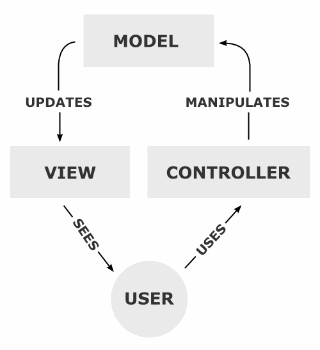
\includegraphics[scale=0.5]{MVC-Process}

\end{figure}

\end{frame}


\section{JavaBeans}


\begin{frame}

\begin{center}
\textbf{{\Huge JavaBeans}}
\end{center}

\end{frame}


\begin{frame}

\frametitle{JavaBeans}

{\Large Dit zijn herbruikbare software componenten voor Java. In de praktijk wilt dit zeggen dat JavaBeans klassen zijn die voldoen aan een bepaalde conventie.\\~\\
Een JavaBean\\

\begin{enumerate}
  \item is serializable\\
  \item heeft \textbf{minstens} een 0-argument constructor\\
  \item heeft getter \textbf{en/of} setter methodes voor zijn fields
\end{enumerate}
}
\end{frame}


\begin{frame}[fragile]

\frametitle{JavaBean en EL}

{\Large Als je een JavaBean set als Attribute van een request kan je in
de JSP een field van de JavaBean aanspreken met de volgende syntax

\begin{verbatim}
${requestAttribuut.attribuut}
\end{verbatim}
}

\end{frame}


\begin{frame}[fragile]

\frametitle{JavaBean en EL}

{\Large Bijvoorbeeld een JavaBean van klasse Auto met een field 'merk'\\
Servlet code
\begin{verbatim}
Auto auto = new Auto("Ford");
request.setAttribute("auto", auto);
\end{verbatim}

JSP code
\begin{verbatim}
${auto.merk}
\end{verbatim}

HTML code
\begin{verbatim}
Ford
\end{verbatim}
}

\end{frame}


\begin{frame}[fragile]

\frametitle{JavaBean en EL}

{\Large Dit werkt omdat EL het volgende doet bij een JavaBean object\\~\\

EL vertaalt de volgende JSP code 
\begin{verbatim}
${auto.merk}
\end{verbatim}
Naar de volgende Java code
\begin{verbatim}
auto.getMerk();
\end{verbatim}

Dit is mogelijk omdat een JavaBean een conventie volgt. Als een programmeur
ipv een getMerk() methode een geefHetMerkTerug() methode schrijft zal dit
niet meer lukken.}

\end{frame}


\section{JavaServer Pages Standard Tag Library}


\begin{frame}

\begin{center}
{\Huge \textbf{JavaServer Pages\\Standard Tag Library}}
\end{center}

\end{frame}


\begin{frame}

\frametitle{Waarom JSTL?}

{\Large Om te vermijden dat je alsnog Java code zou gebruiken in JSP biedt JSTL een
reeks tags waarmee je programmatie logica kunt implementeren in een JSP.\\~\\

JSTL is onderverdeeld in verschillende libraries (de naam is dus wel een beetje misleidend) waarvan wij enkel 'core' zullen leren (voorlopig). De andere zijn : internationalization, functions, SQL, XML.}

\end{frame}


\begin{frame}

\frametitle{HTML tags vs JSP tags}

{\Large Het verschil met HTML tags is dat JSTL tags server-sided tags zijn. Deze worden dus op de server geparsed bij de convertie van een JSP naar een Java Class ( de Web Container maakt van elke JSP een Java Class die de HTML genereerd voor de response )}

\end{frame}


\begin{frame}

\frametitle{Maintenance}

{\Large JSP's maken \textbf{maintenance} makkelijker en zorgen voor een duidelijkere splitsing tussen
Java code en JSP code.\\~\\

\textit{Software maintenance} gebeurt na de initi\"ele deployment van het product.
Het omvat het corrigeren van fouten, het aanpassen van functionaliteiten en het 
toevoegen van nieuwe functionaliteiten. Het succes van een software product hangt
voor een groot deel af van de \textbf{'maintainability'}. }

\end{frame}


\begin{frame}

\frametitle{JSTL toepassen in JSP}

{\Large Allereerst moet je de libraries toevoegen aan je website. \\~\\

\begin{enumerate}
  \item Maak een folder 'lib' onder WEB-INF
  \item importeer de jstl.jar en standard.jar (deze importeer je best
        vanuit de gelijknamige folder in het ServletAndJSPExampleProject)
\end{enumerate}
}

\end{frame}


\begin{frame}[fragile]

\frametitle{JSTL toepassen in JSP}

{\Large Daarna moet je duidelijk maken dat de core library van 
JSTL wilt gebruiken in je JSP met de volgende taglib directive.

\begin{verbatim} 

<%@ taglib 
uri="http://java.sun.com/jsp/jstl/core" 
prefix="c" %>

\end{verbatim}
}

\end{frame}


\begin{frame}[fragile]

\frametitle{De tags}

{\Large Een tag om loops te maken

\begin{verbatim}
<c:forEach> repeat me! </c:forEach>
\end{verbatim}

Een tag om 'if statements' te maken

\begin{verbatim}
<c:if test=""> 
Voer mij uit als de test true geeft 
</c:if>
\end{verbatim}
}

\end{frame}


\begin{frame}[fragile]

\frametitle{De tags}

{\Large Een tag om een 'switch' te maken

\begin{verbatim}
<c:choose>
  <c:when test=""> 
  Voer mij uitals de test true geeft 
  </c:when>
</c:choose>
\end{verbatim}

Een tag om tekst letterlijk op het scherm te krijgen

\begin{verbatim}
<c:out value="iets wat niet geparsed wordt"/>
\end{verbatim}
}

\end{frame}


\begin{frame}[fragile]

\frametitle{De tags}

{\Large Een tag om url's te maken en parameters toe te voegen aan de query string

\begin{verbatim}
<c:url value="/anAbsoluteURL"/>
\end{verbatim}

Een tag om externe JSP's te importeren in de huidige JSP

\begin{verbatim}
<c:import url="eenURLNaarEenJSP>
\end{verbatim}
}

\end{frame}


\begin{frame}[fragile]

\frametitle{De tags}

{\Large Een tag om een variabele aan te maken die je elders in de JSP kunt aanspreken

\begin{verbatim}
<c:set var="variabeleNaam" 
value="variabeleWaarde"/>
\end{verbatim}
}

\end{frame}


\begin{frame}

\frametitle{URL tag revisited}

{\LARGE \begin{itemize}
  \item relatieve URL : URL zonder '/' voor
  \item absoluut URL : URL met '/' voor
\end{itemize}}

\end{frame}


\begin{frame}[fragile]

\frametitle{Probleem bij relatieve URL}

{\Large 

Je begeeft je op de volgende URL

\begin{verbatim}
http://localhost:8080/MijnWebSite/homePage
\end{verbatim}

in homePage.jsp staat een relatieve URL

\begin{verbatim}
images/picture.png
\end{verbatim}
}

\end{frame}


\begin{frame}[fragile]

{\Large De browser zal alles na de laatste '/' verwijderen en de relatieve URL daarachter plaatsen

\begin{verbatim}
http://localhost:8080/
MijnWebSite/images/picture.png
\end{verbatim}

SUCCES!}

\end{frame}


\begin{frame}[fragile]

{\Large Maar wat je start op de volgende URL

\begin{verbatim}
http://localhost:8080/MijnWebSite/
homePage/eenView
\end{verbatim}

En in eenView.jsp staat dezelfde relatieve URL met als resultaat dus

\begin{verbatim}
http://localhost:8080/MijnWebSite/
homePage/images/picture.png
\end{verbatim}

FAILURE!}

\end{frame}


\begin{frame}[fragile]

\frametitle{probleem bij absoluut URL}

{\Large 

Je begeeft je op de volgende URL

\begin{verbatim}
http://localhost:8080/MijnWebsite/homePage
\end{verbatim}

In homePage.jsp staat een absoluut URL

\begin{verbatim}
/images/picture.png
\end{verbatim}
}

\end{frame}


\begin{frame}[fragile]

{\Large De browser zal nu naar de volgende URL gaan

\begin{verbatim}
http://localhost:8080/images/picture.png
\end{verbatim}

FAILURE!}

\end{frame}


\begin{frame}

\frametitle{context path}

{\Large Het onderdeel '/MijnWebSite' is de naam van je website op de webserver.\\
Dit is het \textbf{context path} van je website.\\~\\

Het is dit context path dat de \textless c:url\textgreater\ tag automatisch voor je 
absoluut URL zet. Zodoende zal je site blijven werken ook al verander
je van context path.}

\end{frame}


\begin{frame}

\frametitle{opdracht}

{\Large Probeer te achterhalen hoe je deze tags toepast door het voorbeeldproject te bestuderen. Elke tag is in dit project verwerkt. \\~\\

Pas dan deze tags toe op je ERP project\\ (waar dit nuttig is).\\~\\

Als je er echt niet aan uit kunt vraag je het.}

\end{frame}


\end{document}
